\documentclass{article} 
\usepackage{nips_2018}
\usepackage{mathtools}
\usepackage{xfrac}
\usepackage{amsfonts}
\usepackage{amsthm}
\usepackage{subfig}
\usepackage{hyperref}
\usepackage{xcolor}

\usepackage{times}
\usepackage{float}

\graphicspath{{./graphics/}}
\usepackage{subfig}

\newtheorem{theorem}{Theorem}
\newtheorem{lemma}{Lemma}

\begin{document}

\title{Supplementary materials for the paper ``Uncertainty propagation in neural networks for sparse coding''}

%\author{ }

\maketitle

\section{Proofs}

\begin{lemma}[Propagation of a Gaussian distribution through soft thresholding]
\label{thm:soft_thresholding}
The distribution of $x^*$ can be parametrised by the probability of being zero, $\omega^*$, the mean $m^*$ and the variance $v^*$ of the truncated Gaussian distribution.
\end{lemma}
\begin{proof}

The probability of a zero $\omega^*$ equals to the probability mass of the original distribution from the interval $[-\lambda, \lambda]$
\begin{align}
\begin{split}
\omega^* &=\operatorname{P}(x^*=0) = \operatorname{P}(x \in [-\lambda, \lambda]) \\
&= \Phi\left(\frac{\lambda-m}{\sqrt{v}}\right) - \Phi\left(\frac{-\lambda-m}{\sqrt{v}}\right).
\end{split}
\end{align}
where $\Phi(\cdot)$ is the standard Gaussian cumulative distribution function.

The soft thresholding function shifts elements that are greater than $\lambda$  or less than $-\lambda$ towards~$0$. Let $\psi(\cdot)$ denote the density of the soft-thresholded distribution on $x^* \neq 0$, $\phi(\cdot)$ denote the density of the original Gaussian distribution on $x$. Then the first moment of $x^* \neq 0$ is:

\begin{align}
\label{eq:thr_first_moment}
\begin{split}
m^* &= \int_{-\infty}^{+\infty}x\psi(x)dx= \int_{-\infty}^{0}x\phi(x-\lambda)dx \\
&{} + \int_{0}^{+\infty}x\phi(x+\lambda)dx,
\end{split}
\end{align}
where
\begin{align}
&\int_{-\infty}^{0}x\phi(x-\lambda)dx = -\frac{\sqrt{v}}{\sqrt{2\pi}} \exp\left\{\frac{-(\lambda+m)^2}{2v}\right\} \nonumber\\
&{} + (\lambda+m)\Phi\left(-\frac{\lambda+m}{\sqrt{v}}\right)\\
&\int_{0}^{+\infty}x\phi(x+\lambda)dx = \frac{\sqrt{v}}{\sqrt{2\pi}} \exp\left\{\frac{-(m - \lambda)^2}{2v}\right\}\nonumber\\
& + (m - \lambda)\left(1 - \Phi\left(-\frac{\lambda-m}{\sqrt{v}}\right)\right)
\end{align}

The second moment of $x^* \neq 0$ is given as
\begin{align}
\label{eq:thr_second_moment}
\begin{split}
s &= \int_{-\infty}^{+\infty}x^2\psi(x)dx = \int_{-\infty}^{0}x^2\phi(x-\lambda)dx \\
&{}+ \int_{0}^{+\infty}x^2\phi(x+\lambda)dx,
\end{split}
\end{align}
where
\begin{align}
\begin{split}
&\int_{-\infty}^{0}x^2\phi(x-\lambda)dx = \\
&-\frac{\sqrt{v}}{\sqrt{2\pi}} (\lambda+m)\exp\left\{\frac{-(\lambda+m)^2}{2v}\right\}\\
& + (\sigma^2 + (\lambda+m)^2)\Phi\left(-\frac{\lambda+m}{\sqrt{v}}\right)
\end{split}\\
\begin{split}
&\int_{0}^{+\infty}x^2\phi(x+\lambda)dx = \\
&\frac{\sqrt{v}}{\sqrt{2\pi}} (m - \lambda)\exp\left\{\frac{-(m - \lambda)^2}{2v}\right\}\\
& + (\sigma^2 + (m - \lambda)^2)\left(1 - \Phi\left(\frac{\lambda -m}{\sqrt{v}}\right)\right)
\end{split}
\end{align}

The resulting variance is then
\begin{equation}
v^* = s- (m^*)^2
\end{equation}
\end{proof}

\begin{lemma}[Moments of a spike and slab distribution]
\label{thm:moments_spsl}
Let a random variable $\xi$ have a spike and slab distribution with probability of spike $\omega$, slab mean $m$ and slab variance $v$. Then its moments are
\begin{subequations}
\begin{align}
\mathbb{E}\xi &= (1-\omega)m \\
\operatorname{Var}\xi & = (1-\omega)(v + \omega m^2)
\end{align}
\end{subequations}
\end{lemma}

\begin{proof}
\begin{align*}
\begin{split}
\mathbb{E}\xi &= \int x \big(\omega \delta_0(x) + (1 - \omega)\mathcal{N}(x; m, v)\big)dx \\
& = \omega \int x \delta_0(x)dx + (1 - \omega)\int x \mathcal{N}(x; m, v)dx \\
& = (1-\omega)m \\
\mathbb{E}\xi^2 &= \int x^2 \big(\omega \delta_0(x) + (1 - \omega)\mathcal{N}(x; m, v)\big)dx \\
& = \omega \int x^2 \delta_0(x)dx + (1 - \omega)\int x^2 \mathcal{N}(x; m, v)dx \\
& = (1-\omega)(v + m^2) \\
\operatorname{Var}\xi &= \mathbb{E}\xi^2 - \left(\mathbb{E}\xi\right)^2 = (1-\omega)(v + \omega m^2)
\end{split}
\end{align*}
\end{proof}


\begin{lemma}[Product of a Gaussian matrix and a spike and slab vector]
  \label{thm:matrix_vector}
Let $\mathbf{S} \in \mathbb{R}^{D \times D}$ be a matrix of independent Gaussian-distributed random variables: $s_{d'd''} \sim \mathcal{N}(m^s_{d'd''}, v^s_{d'd''})$, and $\widehat{\boldsymbol\beta }\in \mathbb{R}^D$ be a vector with spike-and-slab distributed variables: $\widehat{\beta}_d \sim \omega_d \delta_0 + (1 - \omega_d)\mathcal{N}(m_d, v_d)$. The components of the matrix $\mathbf{S}$ and the vector $\widehat{\boldsymbol\beta}$ are mutual independent. Let $\mathbf{e} \in \mathbb{R}^{D}$ denote the product $\mathbf{S} \widehat{\boldsymbol\beta}$. Then the marginal mean and variance of elements $e_d$ of the vector $\mathbf{e}$ are:
\begin{subequations}
\begin{align}
 \mathbb{E}e_d &= \sum_{d'=1}^D m^s_{dd'}(1-\omega_{d'})m_{d'}, \\
 \begin{split}
 \operatorname{Var}e_d &= \sum_{d'=1}^D [(m^s_{dd'})^2(1-\omega_{d'})^2v_{d'} \\
 & {}+ (1-\omega_{d'})^2(m_{d'})^2v^s_{dd'} + v^s_{dd'}(1-\omega_{d'})^2v_{d'}].
 \end{split}
 \end{align}
\end{subequations}
 \end{lemma}
 \begin{proof}
\begin{flalign*}
	\mathbb{E}e_d &= \sum_{d'=1}^D \mathbb{E}[s_{dd'}\widehat{\beta}_{d'}]  = \sum_{d'=1}^D m^s_{dd'}\mathbb{E}\widehat{\beta}_{d'}\\
	\operatorname{Var}e_d &= \sum_{d'=1}^D \operatorname{Var}[s_{dd'}\widehat{\beta}_{d'}] = \sum_{d'=1}^D [(\mathbb{E}s_{dd'})^2 \operatorname{Var}\widehat{\beta}_{d'} \\
	&{}+ (\mathbb{E}\widehat{\beta}_{d'})^2 \operatorname{Var}s_{dd'} + \operatorname{Var}\widehat{\beta}_{d'} \operatorname{Var}s_{dd'}]
\end{flalign*}
where $\mathbb{E}\widehat{\beta}_{d'}$ and $\operatorname{Var}\widehat{\beta}_{d'}$ are computed according to Lemma~\ref{thm:moments_spsl}.
 \end{proof}
 
\section{Approximation quality}
\label{sec:approx_quality}

\begin{figure}[!t]
\subfloat[Approximation of the \newline product of Gaussians]{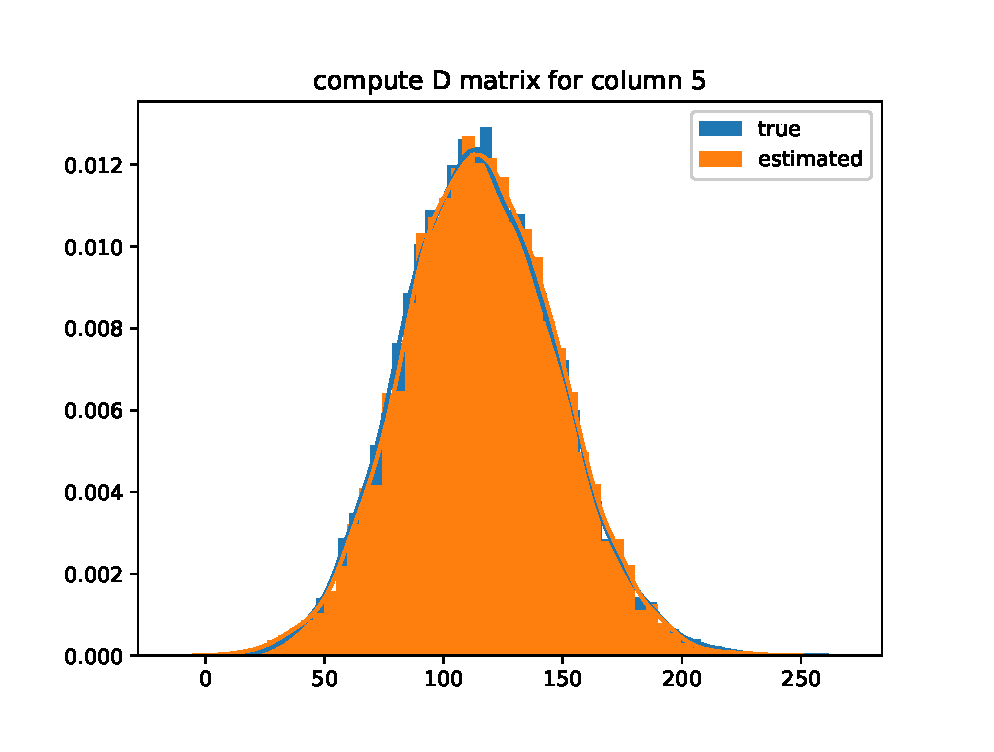
\includegraphics[width=0.5\columnwidth]{d_testing}\label{fig:d_testing}}
%\label{fig:d_testing}
\subfloat[Approximation of the propagation through soft thresholding]{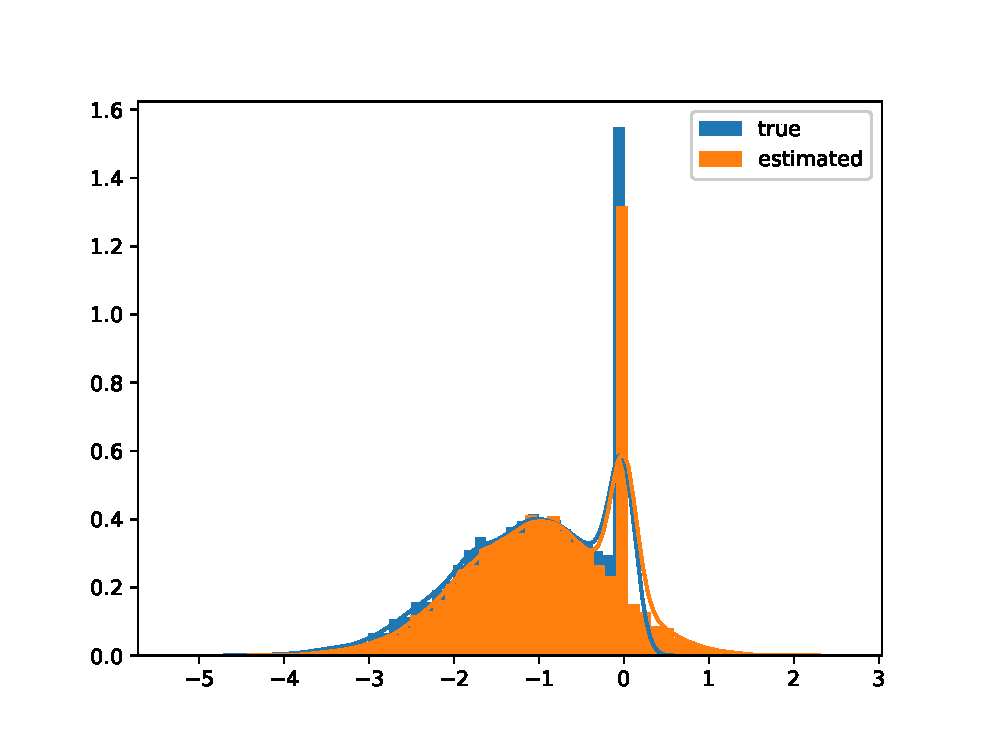
\includegraphics[width=0.5\columnwidth]{z_new_testing}\label{fig:z_new_testing}}
\caption{Approximations of the Bayesian \textsc{lista}}
%\label{fig:z_new_testing}
\end{figure}

We have used two approximations in forward propagation of uncertainty. First, at the step (\ref{eq:l_dense_layer}) during the computation of $\mathbf{e}_l$, a Gaussian matrix is multiplied by a spike and slab vector and their product is approximated with the Gaussian distribution. Second, at the steps (\ref{eq:thr_first}) and (\ref{eq:l_thr}) the result of soft thresholding of a Gaussian vector is approximated with the spike and slab distribution. In this section we demonstrate that these approximations are close to the real distributions.

Figure \ref{fig:d_testing} demonstrates the comparison of the sampled distribution and approximated distribution for Lemma \ref{thm:matrix_vector}. For the sampled distribution, $10000$ values are sampled from the Gaussian matrix and the spike and slab vector and their product is computed, then one of the dimensionalities is plotted. The parameters of the approximated distribution is computed according to Lemma \ref{thm:matrix_vector}.

Figure \ref{fig:z_new_testing} demonstrates the comparison of the sampled distribution and approximated distribution for Lemma \ref{thm:soft_thresholding}. For the sampled distribution, $10000$ values are sampled from the Gaussian vector and propagated through soft thresholding, then one of the dimensionalities is plotted. The parameters of the approximated distribution is computed according to Lemma \ref{thm:soft_thresholding}.

\section{Derivation for the normalisation constant}
When the likelihood term for a single data point is incorporated into the approximating distribution $q$, the normalisation constant of $q$ is expressed as
\begin{equation}
\label{eq:Z}
Z = \int \prod_{d=1}^{D} \mathcal{N}(\beta_d | f(\mathbf{y} ; \mathbf{S}, \mathbf{W}, \lambda), \gamma^{-1}) q(\mathbf{W}, \mathbf{S}, \gamma, \eta) \mathrm{d}\mathbf{W} \mathrm{d}\mathbf{S} \mathrm{d}\gamma \mathrm{d}\eta
\end{equation}
We sample $\mathbf{W}$, $\mathbf{S}$ from $q$ and get $\widehat{\boldsymbol\beta} = \widehat{\boldsymbol\beta}_L = f(\mathbf{y} ; \mathbf{S}, \mathbf{W}, \lambda)$, that is the output from the network and approximate with the spike and slab distribution with the parameters $\boldsymbol\omega^{\widehat{\boldsymbol\beta}}$, $\mathbf{m}^{\widehat{\boldsymbol\beta}}$, and $\mathbf{v}^{\widehat{\boldsymbol\beta}}$
\begin{align}
Z &\approx \int \prod_{d=1}^{D} \mathcal{N}\left(\beta_d | \widehat{\beta}_d, \gamma^{-1}\right) \left(\omega^{\widehat{\boldsymbol\beta}}_d \delta_0\left(\widehat{\beta}_d\right) + \left(1 - \omega^{\widehat{\boldsymbol\beta}}_d\right)\mathcal{N}\left(\widehat{\beta}_d | m^{\widehat{\boldsymbol\beta}}_d, v^{\widehat{\boldsymbol\beta}}_d\right)\right) \text{Gam} \left(\gamma_d; \alpha^\gamma, \beta^\gamma\right)\mathrm{d}\widehat{\boldsymbol\beta} \mathrm{d}\gamma  \nonumber\\
& = \prod_{d=1}^{D} \left[\omega^{\widehat{\boldsymbol\beta}}_d \int \mathcal{N}\left(\beta_d | 0, \gamma^{-1}\right)  \text{Gam} \left(\gamma; \alpha^\gamma, \beta^\gamma\right) d\gamma  \nonumber \right.\\
&\quad + \left(1 - \omega^{\widehat{\boldsymbol\beta}}_d\right)\int \mathcal{T}\left(\beta_d | \widehat{\beta}_d, \beta^\gamma / \alpha^\gamma, 2\alpha^\gamma\right) 
\left. \vphantom{\int}  \mathcal{N}\left(\widehat{\beta}_d | m^{\widehat{\boldsymbol\beta}}_d, v^{\widehat{\boldsymbol\beta}}_d\right) \mathrm{d}\widehat{\boldsymbol\beta}_d\right]  \nonumber\\
\label{eq:Z_approx}
& \approx \prod_{d=1}^D \left[\omega^{\widehat{\boldsymbol\beta}}_d  \mathcal{T}\left(\beta_d | 0, \beta^\gamma / \alpha^\gamma, 2\alpha^\gamma\right) + \vphantom{m^{\widehat{\boldsymbol\beta}}_d} \left(1 - \omega^{\widehat{\boldsymbol\beta}}_d\right)\mathcal{N}\left(\beta_d | m^{\widehat{\boldsymbol\beta}}_d,  \beta^\gamma / (\alpha^\gamma - 1) + v^{\widehat{\boldsymbol\beta}}_d\right)\right],
\end{align}
where we have approximated the Student's t density $\mathcal{T}\left(\beta_d | \widehat{\beta}_d, \beta^\gamma / \alpha^\gamma, 2\alpha^\gamma\right)$ with a Gaussian density with the same mean and variance. The Student's t density can be parametrised in different ways. In this work the following parametrisation is used
\begin{equation}
\mathcal{T}(x; \mu, \beta, \nu) = \frac{\Gamma\left(\frac{\nu + 1}{2}\right)}{\Gamma\left(\frac{\nu}{2}\right)\sqrt{\pi \nu \beta}} \left(1 + \frac{(x - \mu)^2}{\nu\beta}\right)^{-\frac{\nu + 1}{2}}
\end{equation}
where $\Gamma(\cdot)$ denotes the Gamma function.

\section{Hyperparameter optimisation}
The only hyperparameter in the proposed Bayesian \textsc{lista} is the shrinkage parameter $\lambda$. It can be optimised using the Type II maximum likelihood procedure. The Type II likelihood, i.e. the evidence $p(\boldsymbol\beta | \mathbf{y}, \lambda)$, of the Bayesian \textsc{lista} is equal to the normalisation constant $Z$ (\ref{eq:Z}) computed for the whole training dataset $\boldsymbol\beta$. Given the approximation~(\ref{eq:Z_approx}) the optimal hyperparameter $\lambda$ can be found by a gradient-based optimiser.

\section{Performance measures}
\textsc{nmse} for a batch of data $\{\boldsymbol\beta^{(n)}\}_{n=1}^{N}$ and estimates $\{\widehat{\boldsymbol\beta}^{(n)}\}_{n=1}^{N}$ is computed as
\begin{equation}
\text{\textsc{nmse}} = \frac{1}{N}\sum\limits_{n=1}^N\sqrt{\frac{\sum\limits_{d=1}^D\left(\widehat{\beta}_{d}^{(n)} - \beta_d^{(n)}\right)^2}{\sum\limits_{d=1}^D\left(\beta_{d}^{(n)}\right)^2}}
\end{equation}
In sparse coding it is also important to obtain the correct locations of spikes (i.e zeros) and slabs (i.e. non-zeros) in the estimates. The problem is therefore viewed as a skewed two-class classification problem where the number of spikes is higher than the number of slabs. F measure is used to evaluate the accuracy of such problems. It is defined as the harmonic mean of precision and recall
\begin{equation}
\text{F measure} = 2\dfrac{\text{precision}\cdot\text{recall}}{\text{precision} + \text{recall}},
\end{equation}
where precision is the fraction of estimated slab locations that are correct, recall is the fraction of true slab locations among all predicted slab locations.

\section{Posterior estimation for the \textsc{mnist} data}
Figure~\ref{fig:posterior_samples} shows samples from the posterior for one of the validation data points and Figure \ref{fig:posterior_distribution} shows the parameters of this posterior.

\begin{figure}[t]
\centering
\subfloat[]{\includegraphics[width=0.33\columnwidth]{posterior_sample_0}}~
\subfloat[]{\includegraphics[width=0.33\columnwidth]{posterior_sample_1}}~
\subfloat[]{\includegraphics[width=0.33\columnwidth]{posterior_sample_2}}
\caption{Samples from the posterior for an image of the digit 7.}
\label{fig:posterior_samples}
\end{figure}

\begin{figure}[t]
\centering
\subfloat[$\beta$ posterior mean]{\includegraphics[width=0.33\columnwidth]{posterior_mean}}~
\subfloat[$\beta$ posterior std]{\includegraphics[width=0.33\columnwidth]{posterior_std}}~
\subfloat[$\beta$ posterior spike indicator]{\includegraphics[width=0.33\columnwidth]{posterior_spike_indicator}}
\caption{Posterior parameters for an image of the digit 7.}
\label{fig:posterior_distribution}
\end{figure}


%\bibliography{bibliography}
%\bibliographystyle{icml2018}

\end{document}
